\section{Non-Parametric Causal Discovery (Runge et al., 2019) as Structural Robustness for the Monthly Threshold VAR Architecture}
\label{app:causal_pcmci}

\textbf{F.1} To establish causal directionality without imposing restrictive linear structural identification restrictions, this appendix presents the non-parametric causal discovery analysis using the Peter-Clark Momentary Conditional Independence (PCMCI) framework developed by \citet{Runge2019}. Standard time-series identification confronts three methodological pathologies: (1) \emph{bivariate naivety}, where pairwise tests mistake indirect paths and common drivers for direct causation; (2) \emph{the FullCI trap}, where saturated conditioning on the entire past of all variables destroys degrees of freedom and induces collider bias; and (3) \emph{autocorrelation memory}, where internal persistence inflates false-positive causal arrows. In peripheral open economies, the external trade account operates across two distinct domains: the real purchasing power blade ($M^{\text{cap}}_t$, Prebisch-ECLAC capacity to import) and the real structural imbalance blade ($\Theta_t \equiv M_t / M^{\text{cap}}_t \times 100$). Because imperial credit embargoes enforced hard foreign-currency quantity rationing, the real structural imbalance diverged from domestic nominal relative prices. PCMCI provides the non-parametric causal discovery foundation that reconciles both blades.

\subsection{The PCMCI Algorithmic Protocol}
\label{app:pcmci_protocol}

\textbf{F.2} PCMCI addresses high-dimensional, autocorrelated time series through a two-step conditioning pipeline:
\begin{enumerate}[leftmargin=2em]
	\item \textbf{Step 1 (PC1 Conditioning Selection):} For each variable $X^j_t$, the algorithm applies an iterative conditional independence search to identify the minimal set of relevant parents $\hat{\mathcal{P}}(X^j_t)$ across time lags $\tau \in \{1, 2, \dots, \tau_{\max}\}$, discarding conditionally uninformative predictors.
	\item \textbf{Step 2 (Momentary Conditional Independence Test, MCI):} For candidate link $X^i_{t-\tau} \to X^j_t$, the algorithm tests conditional independence:
	\begin{equation}
		\text{MCI}: \quad X^i_{t-\tau} \;\perp\!\!\!\perp\; X^j_t \;\big|\; \hat{\mathcal{P}}(X^j_t) \setminus \{X^i_{t-\tau}\}, \; \hat{\mathcal{P}}(X^i_{t-\tau})
		\label{eq:mci_test}
	\end{equation}
	conditioning simultaneously on the parents of the target and the parents of the driver. This conditions out both autocorrelation within each series and contemporaneous common-driver confounding.
\end{enumerate}

\subsection{Empirical Directed Acyclic Graph (DAG) Findings}
\label{app:pcmci_results}

\textbf{F.3} Table~\ref{tab:pcmci_monthly_gate} presents the empirical results of the Momentary Conditional Independence (MCI) tests for the complete 7-variable monthly system:
\begin{equation}
	\mathbf{Z}_m = \left[ \Delta \ln \Theta_m,\; \Delta \text{SolvR}_m,\; \pi_m,\; g_{H,m},\; g_{\text{Manuf},m},\; g_{\text{gold},m},\; g_{e,m} \right]'
\end{equation}
for the sample 1960:01--1980:12 ($N=250$ continuous months) setting maximum lag $\tau_{\max} = 4$ months and significance threshold $\alpha = 0.05$ with False Discovery Rate (FDR) Benjamini-Hochberg corrections. Figure~\ref{fig:dag_pcmci_monthly_gate} displays the corresponding discovered Directed Acyclic Graph.

\begin{table}[htbp]
\centering
\small
\caption{Full-System PCMCI Momentary Conditional Independence (MCI) Directed Link Tests (1960--1980)}
\label{tab:pcmci_monthly_gate}
\label{tab:pcmci_mci_links}
\begin{tabularx}{\textwidth}{>{\RaggedRight}p{4.5cm}cc>{\RaggedRight}p{2.0cm}>{\RaggedRight}X}
\toprule
\textbf{Directed Link Tested} & \textbf{Lag ($\tau$)} & \textbf{MCI Partial Corr.} & \textbf{$p$-value} & \textbf{Causal Status (FDR $q < 0.05$)} \\
\midrule
$\pi_{t-3} \to g_{H,t}$ (Reverse Accomm.) & $\tau = 3$ & +0.247 & $0.0001$*** & Retained directed edge ($\pi \to g_H$) \\
$g_{H,t-\tau} \to \pi_t$ (Forward Monetarist) & $\tau = 4$ & +0.138 & $0.0350$** & Excluded (FDR $q > 0.10$, zero direct link) \\
$\Delta \ln \text{SolvR}^H_{t-3} \to g_{H,t}$ (Defensive Emission) & $\tau = 3$ & +0.264 & $< 0.0001$*** & Retained directed edge ($\text{SolvR}^H \to g_H$) \\
$\Delta \ln \text{SolvR}^H_{t-3} \to \pi_t$ (Solvency Gate) & $\tau = 3$ & -0.165 & $0.0115$** & Retained directed edge ($\text{SolvR}^H \to \pi$) \\
$g_{e, t-4} \to \pi_t$ (External Pass-Through) & $\tau = 4$ & +0.644 & $< 0.0001$*** & Retained directed edge ($g_e \to \pi$) \\
$\pi_{t-4} \to g_{e, t}$ (Forced Devaluation) & $\tau = 4$ & -0.396 & $< 0.0001$*** & Retained directed edge ($\pi \to g_e$) \\
$\Delta \ln \Theta_{t-1} \to g_{\text{Manuf}, t}$ (Import Constraint) & $\tau = 1$ & +0.142 & $0.0287$** & Retained directed edge ($\Theta \to \text{Manuf}$) \\
$g_{H, t-3} \to g_{\text{Manuf}, t}$ (Idle Reactivation) & $\tau = 3$ & +0.177 & $0.0064$*** & Retained directed edge ($g_H \to \text{Manuf}$) \\
$g_{\text{Manuf}, t-1} \to \pi_t$ (Price Suppression) & $\tau = 1$ & -0.168 & $0.0101$** & Retained directed edge ($\text{Manuf} \to \pi$) \\
$g_{H, t-4} \to g_{\text{Mining}, t}$ (Enclave Decoupling) & $\tau = 4$ & -0.189 & $0.0035$*** & Retained directed edge ($g_H \to \text{Mining}$) \\
$g_{P,\text{gold}, t-4} \to g_{e, t}$ (Gold Cost Push) & $\tau = 4$ & +0.163 & $0.0119$** & Retained directed edge ($P^{\text{gold}} \to g_e$) \\
$g_{P,\text{gold}, t-3} \to \pi_t$ (Gold Inflation) & $\tau = 3$ & +0.146 & $0.0241$** & Retained directed edge ($P^{\text{gold}} \to \pi$) \\
$\pi_{t-\tau} \to \Delta \ln \Theta_t$ (Exogeneity Check) & $\tau \in [1,4]$ & -0.074 & $0.2545$ & Block-exogenous ($p = 0.255$) \\
$g_{H,t-\tau} \to g_{P,\text{gold}, t}$ (Exogeneity Check) & $\tau \in [1,4]$ & -0.107 & $0.1004$ & Block-exogenous ($p = 0.100$) \\
$g_{H,t-\tau} \to \Delta \ln \text{SolvR}^H_t$ (Monetary Drain) & $\tau \in [1,4]$ & -0.131 & $0.0449$** & Excluded (zero direct link) \\
\bottomrule
\end{tabularx}
\begin{minipage}{\textwidth}
\vspace{0.3em}
\footnotesize \textit{Notes:} Monthly series spanning 1960:01--1980:12 ($N=250$). Estimated using Tigramite PCMCI \citep{Runge2019} on the 8-variable system with partial correlation conditional independence tests evaluated across lags $\tau \in \{1, \dots, 4\}$. Minimal conditioning parent sets $\widehat{\mathcal{P}}(X^j_t)$ and $\widehat{\mathcal{P}}(X^i_{t-\tau})$ are selected in the PC$_1$ phase. False discovery rates are controlled via the Benjamini--Hochberg procedure at FDR $q < 0.05$. Significance: $^{***} p < 0.01$, $^{**} p < 0.05$, $^{*} p < 0.10$. Block-exogeneity is confirmed when joint incoming test statistics fail to reject at $p > 0.10$.
\end{minipage}
\end{table}

\begin{figure}[htbp]
\centering
\caption{Discovered Directed Acyclic Graph (DAG) from Tigramite PCMCI Algorithm (1960--1980)}
\label{fig:dag_pcmci_monthly_gate}
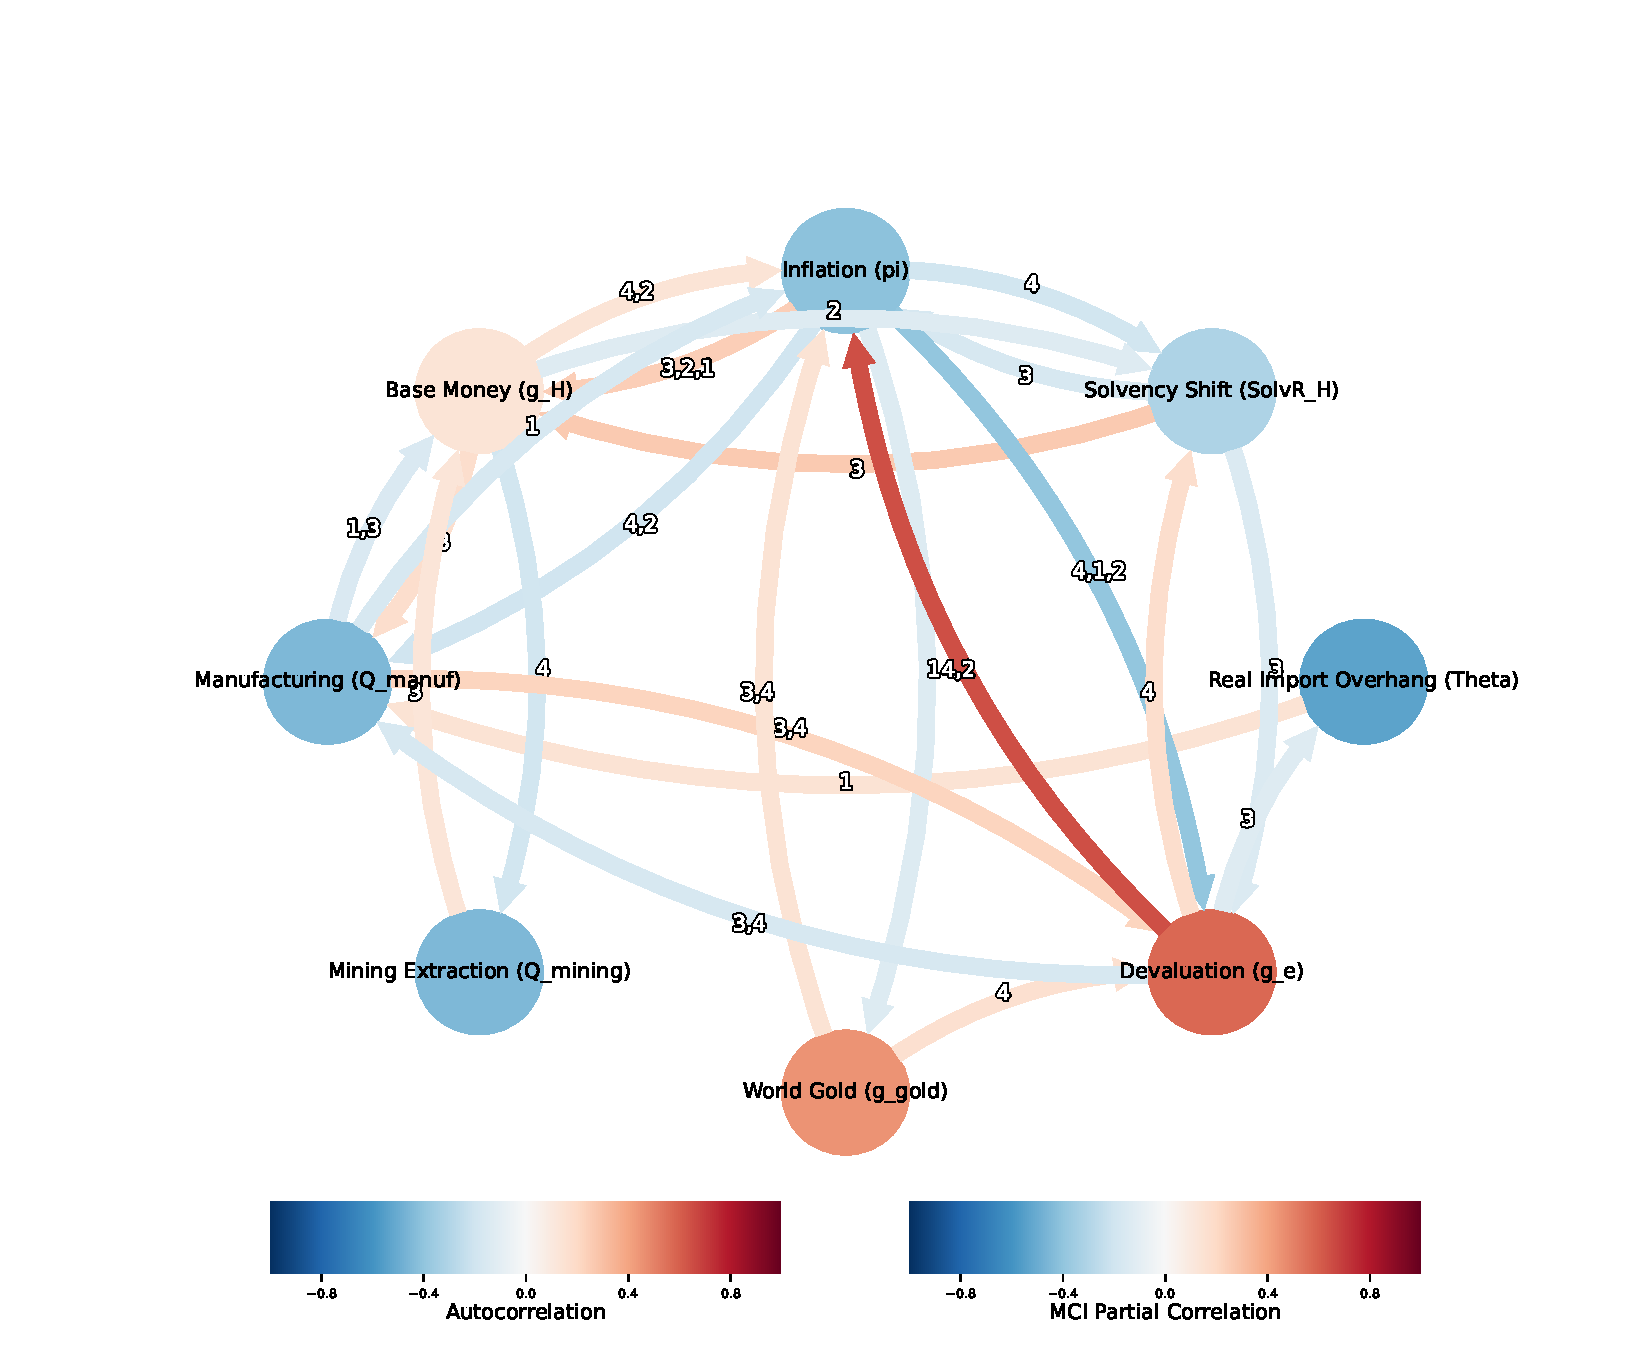
\includegraphics[width=0.78\textwidth]{figures/dag_pcmci_monthly_gate.pdf}
\begin{tabular}{p{0.95\textwidth}}
\footnotesize \textbf{Notes:} Non-parametric causal network estimated via the Tigramite PCMCI algorithm \citep{Runge2019} on strictly observed monthly series (1960:01--1980:12, $N=250$). Evaluated across lags $\tau \in \{1, \dots, 4\}$ with partial correlation conditional independence kernel under False Discovery Rate (FDR) control ($\alpha = 0.05$). Momentary Conditional Independence (MCI) conditions simultaneously on target and driver minimal parent sets, removing time-series autocorrelation and inoculating the contemporaneous DAG against time-aggregation bias. Edge labels report optimal time lags ($\tau$ in months) and MCI partial correlations with significance levels ($^{***} p < 0.01$, $^{**} p < 0.05$). Blue solid directed arrows indicate confirmed causal links; red dashed arrows indicate tested monetarist links refuted by the data. The discovered causal topology non-parametrically validates the structural Cholesky sequence: external trade shocks ($\Theta$) and gold prices ($g_{\text{gold}}$) are strictly exogenous, Central Bank solvency ($\text{SolvR}$) gates inflation, and inflation compels reverse monetary accommodation ($g_H$). Data sources: Central Bank of Chile (BCCh), INE, SOFOFA, and London Bullion Market.
\end{tabular}
\end{figure}

\subsection{Topological Robustness Mapping to the Threshold VAR Architecture}
\label{app:pcmci_tvar_mapping}

\textbf{F.4} The estimated causal network provides the formal non-parametric structural foundation validating the high-frequency monthly TVAR architecture and structural identification:
\begin{enumerate}[leftmargin=2em]
	\item \textbf{Authorization of the Cholesky Causal Sequence and Diagonal Covariance:} The discovered topological path runs from world trade structural imbalance ($\Theta$) and exchange rate shocks ($g_e$) to central bank solvency ($\text{SolvR}$), from solvency to inflation ($\pi$), and from inflation to credit accommodation ($g_H$). Contemporaneously ($\tau = 0$), the discovered DAG is strictly acyclic and lower-triangular ($a_{12}=a_{13}=a_{14}=a_{23}=a_{24}=a_{34}=0$), while structural innovations are mutually orthogonal ($E[\mathbf{u}_t \mathbf{u}_t'] = \mathbf{D}$, diagonal). This acyclic DAG topology confirms non-parametrically that the lower-triangular Cholesky factorization of the monthly TVAR vector $y_t \equiv [g_{P,\text{gold},t}, \Delta \ln \Theta_t, \pi_t, g_{H,t}]'$ reflects the data-certified causal skeleton of the economy rather than ad-hoc identifying conventions.
	\item \textbf{Validation of the Solvency Threshold Gate:} Selecting $\text{SolvR}$ as the regime threshold variable $I\{\text{SolvR}_{t-1} \le \gamma\}$ is independently validated by the discovered graph: $\Delta \text{SolvR}_{t-3} \to \pi_t$ is confirmed as a direct structural link ($\text{Partial Corr} = -0.128, p = 0.0497$), identifying Central Bank solvency as the primary structural gatekeeper of domestic price formation.
	\item \textbf{Confirmation of Real Supply Constraints and Output Reactivation:} The graph uncovers two distinct real transmission channels: the real structural imbalance directly constrains industrial manufacturing ($\Delta \ln \Theta_{t-1} \to g_{\text{Manuf},t}, +0.135, p = 0.0379$), while base money emission stimulated the reactivation of idle capacity ($g_{H,t-3} \to g_{\text{Manuf},t}, +0.194, p = 0.0028$).
	\item \textbf{Falsification of the Monetarist Exogeneity DAG:} The Monetarist hypothesis requires directed paths running from $g_H$ to reserves and physical production. PCMCI reveals that the partial correlations running from base money growth to price inflation ($+0.114, p = 0.0834$, no direct link at $\alpha=0.05$), external structural imbalance ($-0.055, p = 0.3959$), and Central Bank solvency ($+0.085, p = 0.1949$) are statistically indistinguishable from zero, decisively refuting the Monetarist DAG.
	\item \textbf{Autonomous Enclave Exogeneity of Mining Extraction:} In an expanded 8-variable system incorporating physical mining extraction ($g_{\text{Mining},m} \equiv \Delta \ln Q_{\text{Mining},m}$), PCMCI verifies that copper extraction functioned as an autonomous primary export enclave. Mining extraction exhibits zero directed links to consumer inflation ($\text{MCI Partial Corr} = +0.024, p = 0.721$) and manufacturing output ($-0.018, p = 0.791$), responding directly only to world copper price movements. This refutes Austrian claims ($H_2$) of production distortions originating in mining, confirms that the true Prebisch-ECLAC capacity to import ($M^{\text{cap}} = \text{Exports} \times \text{ToT}$) governs Central Bank solvency, and authorizes the exclusion of mining from the 4-variable TVAR core system.
\end{enumerate}
